\subsection{Experiment 3: Comparing the Effect of Varying the Presence of Symbols on the Accuracy of Training} \label{sec:experiment-3}

\subsubsection{Objective}

In the previous experiments, we showed that the presence of symbols improves the effectiveness of recurrent neural networks in learning to perform arithmetic on images of handwritten digits when training using an impoverished dataset. In Section \ref{sec:theory-hypothesis-multi-task-learning} we proposed that this would be the expected behavior due to the beneficial effect of multi-task learning on all tasks being learned by the recurrent networks. In this experiment we attempt to further demonstrate this benefit.
 
Our goal is to show the relationship between the accuracy of the model in classifying the inputs on the intermediate time steps and the accuracy of the same model in producing the correct output for the given mathematical operation. The existence of this relationship should indicate that by correctly classifying the digits, the recurrent neural network is able to create internal features on the first two time steps that are then used on the third time step to perform the arithmetic operation. In the absence of these clear features, the network would rely only on the noisy handwritten inputs.

Besides establishing the relationship between the classification accuracy and the mathematical accuracy of our models, we also to vary the percentage of symbols included with each training example. The expected outcome here is that the higher the percentage of symbols present, the more accurate the classification accuracy will be and in turn the higher the accuracy of performing the arithmetic operation.

\subsubsection{Method}

The architectures constructed for this experiment are the same as the ones used in the previous two experiments. The models accept a sequence of three 28x28 images. The first two images are of the handwritten digits representing the operands of the operation. The third image is that of the operator. The networks output two one-hot vectors. When each of the operands are presented, the model attempts to output a one-hot encoded vector of the value of the operand. When the operator is presented, the network learns to compute and present the output. Two hidden layers are used each containing 512 LSTM units. All four arithmetic operations are used together during training.

The dataset used in Experiment 2 in Section \ref{sec:experiment-2} is replicated into five sets, with some modifications, for use in this experiment. Each combination now includes eight MNIST samples instead of ten, where four are used for training, two for validation and two for testing. This makes the process of varying symbols easier. Each of the five replicas are modified to vary the number of symbols included with each digit combination during training. The first set has no symbols, meaning a vector with all features set to 0.5 is provided as a dummy output for the intermediate classification time steps. The second dataset has 25\% of the MNIST samples in each combination include a symbol whereas the rest use the 0.5 dummy values. The 25\% symbols are distributed such that, out of the four training samples, one has a symbol and the rest do not. The third dataset has 50\% symbols meaning that out of the four training examples per combination two include their corresponding symbols. The fourth dataset has 75\% of the training examples include symbols, meaning three out of four examples per combination include their corresponding symbol. Finally, the fifth dataset, the 100\% symbols dataset, includes symbols for all examples.

Five models were trained each using one of the datasets described above. The networks were trained using the Adam optimizer with the mean square error as the loss function and a learning rate of 0.001. Training is performed over 200 epochs in batches of 100 and the model performing best on the validation set is saved. Each model is trained five times using 5-fold cross-validation where all digit combinations are used. Instead of recording the accuracy of each model as was done in the previous experiments, here we split the accuracy into four new metrics. They are as follows:
\begin{itemize}
	\item False Classification/False Operation \textbf{(FC/FO)}: The percentage of test samples that classify incorrectly during the intermediate time steps that also produce incorrect outputs for the mathematical operation.
	\item False Classification/True Operation \textbf{(FC/TO)}: The percentage of test samples that classify incorrectly during the intermediate time steps that produce correct outputs for the operation.
	\item True Classification/False Operation \textbf{(TC/FO)}: The percentage of test samples that classify correctly during the intermediate time steps that produce incorrect outputs for the operation.
	\item True Classification/True Operation \textbf{(TC/TO)}: The percentage of test samples that classify correctly during the intermediate time steps that also produce correct outputs for the operation.
\end{itemize}

The epoch number that results in the most optimum set of weights for each percentage of symbols used is also recorded, to understand the effect of symbols on the efficiency of training with and without symbols.

\subsubsection{Results}

\begin{table}[p]
	\center
	\caption{A comparison of the mean FC/FO percentage, standard deviation and the p-value of a hypothesis t-Test when compared to the 0\% symbols model.}
	\label{tab:experiment-3-results-table-fcfo}
	\begin{tabular}{ |c|c|c|c| } 
		\hline
		\% Symbols Present & FC/FO (\%) & Standard Deviation  & p-value\\ 
		0\% & 55.8 & 0.063 & NA \\  
		25\% & 39.80 & 0.03 & 0.00493\\  
		50\% & 26.20 & 0.042 & 0.00141 \\  
		75\% & 17.05 & 0.023 & 0.00033\\  
		100\% & 13.60 & 0.012 & 0.00016\\  
		\hline
	\end{tabular}
\end{table}

\begin{table}[p]
	\center
	\caption{A comparison of the mean FC/TO percentage, standard deviation and the p-value of a hypothesis t-Test when compared to the 0\% symbols model.}
	\label{tab:experiment-3-results-table-fcto}
	\begin{tabular}{ |c|c|c|c| } 
		\hline
		\% Symbols Present & FC/TO (\%) & Standard Deviation  & p-value\\ 
		0\% & 37.55 & 0.0672 & NA \\  
		25\% & 27.95 & 0.0387 & 0.0031\\  
		50\% & 11.50 & 0.0351 & 0.00141 \\  
		75\% & 5.40 & 0.0137 & 0.00084\\  
		100\% & 2.45 & 0.0042 & 0.00016\\  
		\hline
	\end{tabular}
\end{table}

\begin{table}[p]
	\center
	\caption{A comparison of the mean TC/FO percentage, standard deviation and the p-value of a hypothesis t-Test when compared to the 0\% symbols model.}
	\label{tab:experiment-3-results-table-tcfo}
	\begin{tabular}{ |c|c|c|c| } 
		\hline
		\% Symbols Present & TC/FO (\%) & Standard Deviation  & p-value\\ 
		0\% & 3.70 & 0.0106 & NA \\  
		25\% & 15.05 & 0.0214 & 0.00183\\  
		50\% & 23.20 & 0.01024 & 0.02209 \\  
		75\% & 13.55 & 0.0107 & 0.00013\\  
		100\% & 8.15 & 0.0158 & 0.01742\\  
		\hline
	\end{tabular}
\end{table}

\begin{table}[p]
	\center
	\caption{A comparison of the mean TC/TO percentage, standard deviation and the p-value of a hypothesis t-Test when compared to the 0\% symbols model.}
	\label{tab:experiment-3-results-table-tcto}
	\begin{tabular}{ |c|c|c|c| } 
		\hline
		\% Symbols Present & TC/TO (\%) & Standard Deviation  & p-value\\ 
		0\% & 2.95 & 0.0166 & NA \\  
		25\% & 17.20 & 0.0148 & 0.00043\\  
		50\% & 39.10 & 0.0853 & 0.00179 \\  
		75\% & 64.00 & 0.0301 & 0.0\\  
		100\% & 75.80 & 0.0213 & 0.0\\  
		\hline
	\end{tabular}
\end{table}

\begin{figure}[p]%
	\centering
	\subfloat[False Classification/False Operation]{{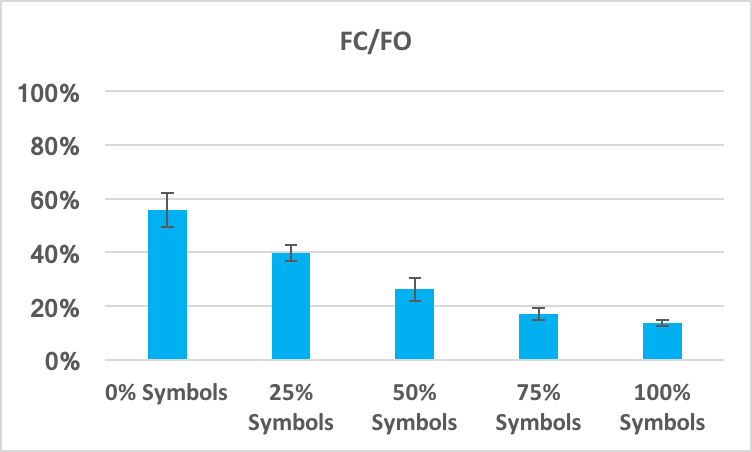
\includegraphics[width=0.5\textwidth]{experiment-3-results-chart-fc-fo} }}\label{fig:experiment-3-results-chart-fc-fo}%
	\subfloat[False Classification/True Operation]{{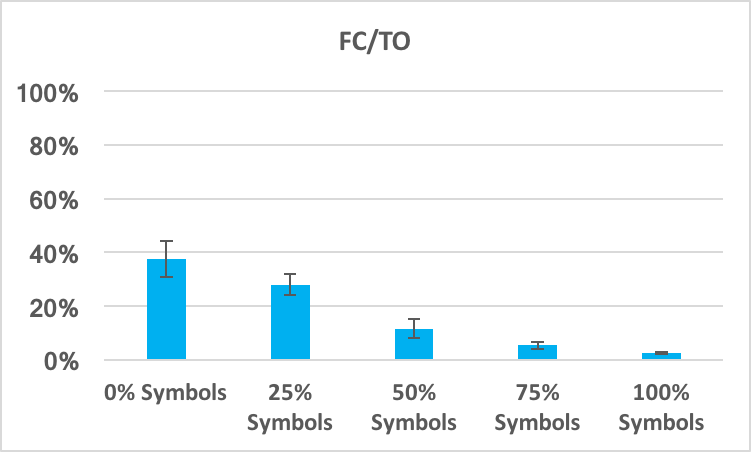
\includegraphics[width=0.5\textwidth]{experiment-3-results-chart-fc-to} }}\label{fig:experiment-3-results-chart-fc-to}%
	
	\subfloat[True Classification/False Operation]{{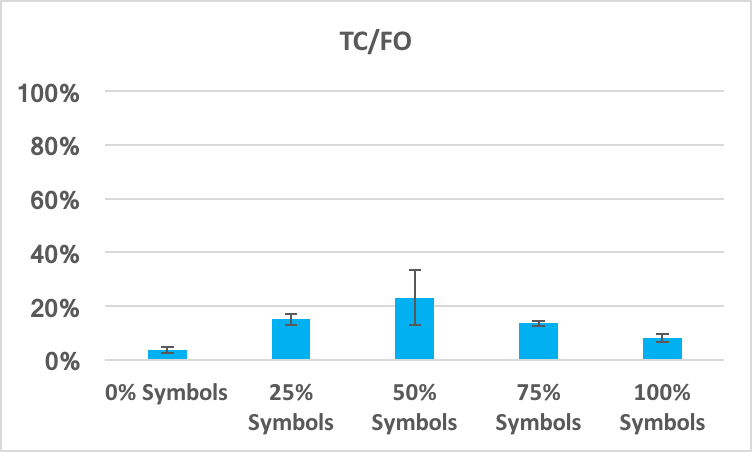
\includegraphics[width=0.5\textwidth]{experiment-3-results-chart-tc-fo} }}\label{fig:experiment-3-results-chart-tc-fo}%
	\subfloat[True Classification/True Operation]{{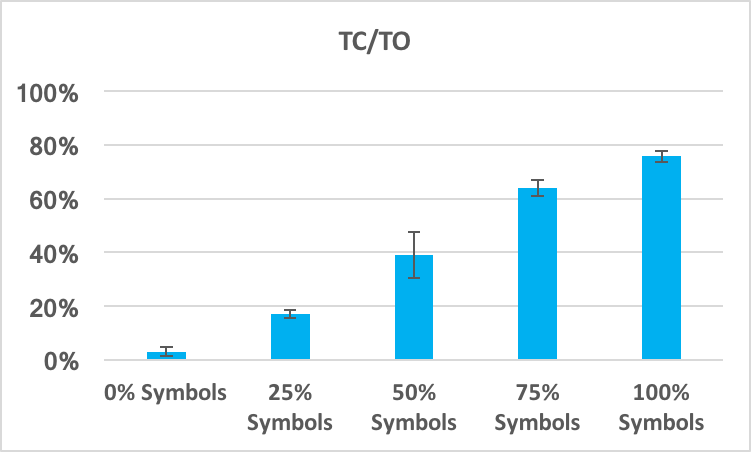
\includegraphics[width=0.5\textwidth]{experiment-3-results-chart-tc-to} }}\label{fig:experiment-3-results-chart-tc-to}%
	\caption{A comparison of the four metrics FC/FO, FC/TO, TC/FO, TC/TO along with their corresponding 95\% confidence intervals for each of the five models developed.}%
	\label{fig:experiment-3-results-chart}%
\end{figure}

Tables \ref{tab:experiment-3-results-table-fcfo} to \ref{tab:experiment-3-results-table-tcto} present the mean FC/FO, FC/TO, TC/FO, TC/TO accuracies for each of the datasets used along with the standard deviations and the p-test score of a hypothesis t-Test compared to the 0\% model. Figure \ref{fig:experiment-3-results-chart} shows the same results presented in graphical form. Table \ref{tab:experiment-3-results-epochs} presents the number of epochs needed for the network to discover the optimum set of weights for each of the five datasets.

\begin{table}[h]
	\center
	\caption{A comparison of the average epoch number at which the optimum weights were discovered for each of the models trained.}
	\label{tab:experiment-3-results-epochs}
	\begin{tabular}{ |c|c| } 
		\hline
		\% Symbols Present & Mean Epoch Number\\ 
		0\% Symbols & 4.2\\  
		25\% Symbols & 10.0\\  
		50\% Symbols & 11.0\\  
		75\% Symbols & 15.8\\  
		100\% Symbols & 38.0\\  
		\hline
	\end{tabular}
\end{table}

\subsubsection{Discussion}

It is clear from Table \ref{tab:experiment-3-results-table-tcto} and Figure \ref{fig:experiment-3-results-chart}(d) that more training examples with symbolic classification data improves the correct output of the operations (TO), particularly when the classification is also correct (TC) (75.8\% of the time with 100\% symbols), and rarely, as shown in Table \ref{tab:experiment-3-results-table-fcto} and Figure \ref{fig:experiment-3-results-chart}(b) when the classification is incorrect (FC) (only 2.45\% of the time with 100\% symbols).

Inversely, as shown in Table \ref{tab:experiment-3-results-table-fcfo} and Figure \ref{fig:experiment-3-results-chart}(a), incorrect output (FO) for a mathematical operator occurs frequently with false classification (FC) (13.6\% of the time with 100\% symbols). It also makes sense that as the percentage of false classifications (FC) declines (due to more symbols in the training set) the percentage of false operation (FO) outputs also declines, because the probability of an operation being performed on the wrong operands decreases.

These results show that the presence of symbols improves the accuracy of classification which in turn improves the accuracy of performing the operation. Classifying the handwritten operands creates an internal representation of the digits that is retained by the LSTM recurrent connections. In the presence of symbols, this representation is learned more consistently for each digit, reducing the variations of the handwritten digits and therefore improving the model's accuracy when performing the operation. This is a recurrent multi-task learning effect that provides beneficial results.

The TC/FO graph of Figure \ref{fig:experiment-3-results-chart}(c) on the other hand says that incorrect operation output (FO) occurs most frequently (23.2\% of the time) when 50\% of the training examples have classification signals and the test examples operands are classified correctly (TC). In fact, the percentage of FO examples is almost as high for TC/FO at 50\%, 75\% and 100\% as they are for FC/FO. This makes it clear that there are limits to the system's ability to get correct operation outputs (TO) even when it has TC for certain examples.

\begin{figure}[t]
	\centering
	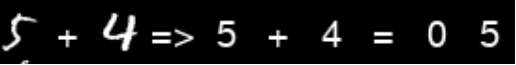
\includegraphics[max width=\textwidth]{tc-fo-example}
	\caption{Example of a TC/FO operation. The operation 5 + 4 is classified correctly, however the output is still false.}
	\label{fig:tc-fo-example}
\end{figure}

This limitation can be due to the fact that the noisy handwritten digits still retain some influence over the network that forces the model to use the noisy inputs for pattern matching instead of the clearer internal representations. Figure \ref{fig:tc-fo-example} shows an example of one of the TC/FO cases trained with 50\% symbols. The handwritten digits are shown along with the result of classification and the result of the operation. The operation is that of 5 + 4. The handwritten digits are classified correctly, however the output of 5 is incorrect. This example shows that the model was still being influenced by the confusing handwritten digits. It might have confused the first operand 5 for the digit 1.

Looking at the results in Table \ref{tab:experiment-3-results-epochs} we see that the more symbols are used the longer it takes for the network to converge onto an optimum decision function. We initially predicted that providing clearer symbols would make the learning process more efficient, but that apparently is not the case. We now understand that without the symbolic information, the gradient descent algorithm will converge to a local minimum early in the training process resulting in the poor classification results and therefore less accurate mathematical operation output. The introduction of more symbols forces the gradient descent algorithm to search longer for an appropriate representation in weight space that is compatible with both the symbol classification and the mathematical operation output.
